\documentclass{beamer}
\usepackage[utf8]{inputenc}
\usepackage{graphicx, epsfig}
\usepackage{amsmath,mathrsfs,amsfonts,amssymb}
\usepackage{floatflt}
\usepackage{epic,ecltree}
\usepackage{mathtext}
\usepackage{fancybox}
\usepackage{fancyhdr}
\usepackage{multirow}
\usepackage{enumerate}
\usepackage{epstopdf}
\usepackage{multicol}
\usepackage{algorithm}
\usepackage[noend]{algorithmic}
\usepackage{tikz}
\usepackage{blindtext}
\usetheme{default}%{Singapore}%{Warsaw}%{Warsaw}%{Darmstadt}
\usecolortheme{default}

\setbeamerfont{title}{size=\Huge}
\setbeamertemplate{footline}[page number]{}

\setbeamertemplate{section in toc}[sections numbered]


\makeatletter
\newcommand\HUGE{\@setfontsize\Huge{35}{40}}
\makeatother    

\setbeamerfont{title}{size=\HUGE}
\beamertemplatenavigationsymbolsempty

% latin bold lower
\newcommand{\ba}{\mathbf{a}} 
\newcommand{\bc}{\mathbf{c}} 
\newcommand{\be}{\mathbf{e}} 
\newcommand{\bh}{\mathbf{h}} 
\newcommand{\bp}{\mathbf{p}} 
\newcommand{\bt}{\mathbf{t}} 
\newcommand{\bs}{\mathbf{s}} 
\newcommand{\bu}{\mathbf{u}} 
\newcommand{\bv}{\mathbf{v}} 
\newcommand{\bw}{\mathbf{w}} 
\newcommand{\bx}{\mathbf{x}} 
\newcommand{\by}{\mathbf{y}} 
\newcommand{\bz}{\mathbf{z}} 

% latin bold upper
\newcommand{\bA}{\mathbf{A}} 
\newcommand{\bB}{\mathbf{B}} 
\newcommand{\bC}{\mathbf{C}} 
\newcommand{\bI}{\mathbf{I}} 
\newcommand{\bJ}{\mathbf{J}} 
\newcommand{\bL}{\mathbf{L}} 
\newcommand{\bM}{\mathbf{M}} 
\newcommand{\bQ}{\mathbf{Q}} 
\newcommand{\bT}{\mathbf{T}} 
\newcommand{\bU}{\mathbf{U}} 
\newcommand{\bV}{\mathbf{V}} 
\newcommand{\bW}{\mathbf{W}} 
\newcommand{\bX}{\mathbf{X}} 
\newcommand{\bY}{\mathbf{Y}} 
\newcommand{\bZ}{\mathbf{Z}} 

% latin cal upper
\newcommand{\cG}{\mathcal{G}} 
\newcommand{\cL}{\mathcal{L}} 
\newcommand{\cN}{\mathcal{N}} 
\newcommand{\cS}{\mathcal{S}} 
\newcommand{\cT}{\mathcal{T}} 
\newcommand{\cW}{\mathcal{W}} 
\newcommand{\cX}{\mathcal{X}} 
\newcommand{\cZ}{\mathcal{Z}} 

% latin bb upper
\newcommand{\bbE}{\mathbb{E}} 
\newcommand{\bbI}{\mathbb{I}} 
\newcommand{\bbP}{\mathbb{P}} 
\newcommand{\bbR}{\mathbb{R}} 

% greek bold lower
\newcommand{\bepsilon}{\boldsymbol{\epsilon}} 
\newcommand{\btheta}{\boldsymbol{\theta}} 
\newcommand{\blambda}{\boldsymbol{\lambda}} 
\newcommand{\bpi}{\boldsymbol{\pi}} 
\newcommand{\bmu}{\boldsymbol{\mu}} 
\newcommand{\bsigma}{\boldsymbol{\sigma}} 
\newcommand{\bphi}{\boldsymbol{\phi}} 

% greek bold upper
\newcommand{\bSigma}{\boldsymbol{\Sigma}} 

\DeclareMathOperator*{\argmin}{arg\,min}
\DeclareMathOperator*{\argmax}{arg\,max}

\newcommand{\createdgmtitle}[1]{\title[\hbox to 56mm{Deep Learning Audio \hfill\insertframenumber\,/\,\inserttotalframenumber}]
	{\vspace{1cm} \\ Deep Learning Audio \\ {\Huge Lecture #1}}
	\author{Pavel Severilov}
	\institute{
	Moscow Institute of Physics and Technology
	} 
	\date{2022}
}

\newcommand\myfootnote[1]{%
  \tikz[remember picture,overlay]
  \draw (current page.south west) +(1in + \oddsidemargin,0.5em)
  node[anchor=south west,inner sep=0pt]{\parbox{\textwidth}{%
      \rlap{\rule{10em}{0.4pt}}\raggedright\scriptsize \textit{#1}}};}

\newcommand\myfootnotewithlink[2]{%
  \tikz[remember picture,overlay]
  \draw (current page.south west) +(1in + \oddsidemargin,0.5em)
  node[anchor=south west,inner sep=0pt]{\parbox{\textwidth}{%
      \rlap{\rule{10em}{0.4pt}}\raggedright\scriptsize\href{#1}{\textit{#2}}}};}
      
\AtBeginSection[]
{
	\begin{frame}{Outline}
		\tableofcontents[currentsection,subsectionstyle=hide]
	\end{frame}
}
\AtBeginSubsection[]{
	\begin{frame}{Outline}
		\tableofcontents[currentsection,currentsubsection]
	\end{frame}
}
\createdgmtitle{6}
\usepackage{tikz}
\usetikzlibrary{arrows,shapes,positioning,shadows,trees}
%--------------------------------------------------------------------------------
\begin{document}
%--------------------------------------------------------------------------------
\begin{frame}[noframenumbering,plain]
%\thispagestyle{empty}
\titlepage
\end{frame}
%=======x
\begin{frame}{Outline}
	\tableofcontents
\end{frame}

\section{Text-to-speech}
%=======
\begin{frame}{Text-to-speech (TTS)}
    \begin{figure}
    	\centering
    	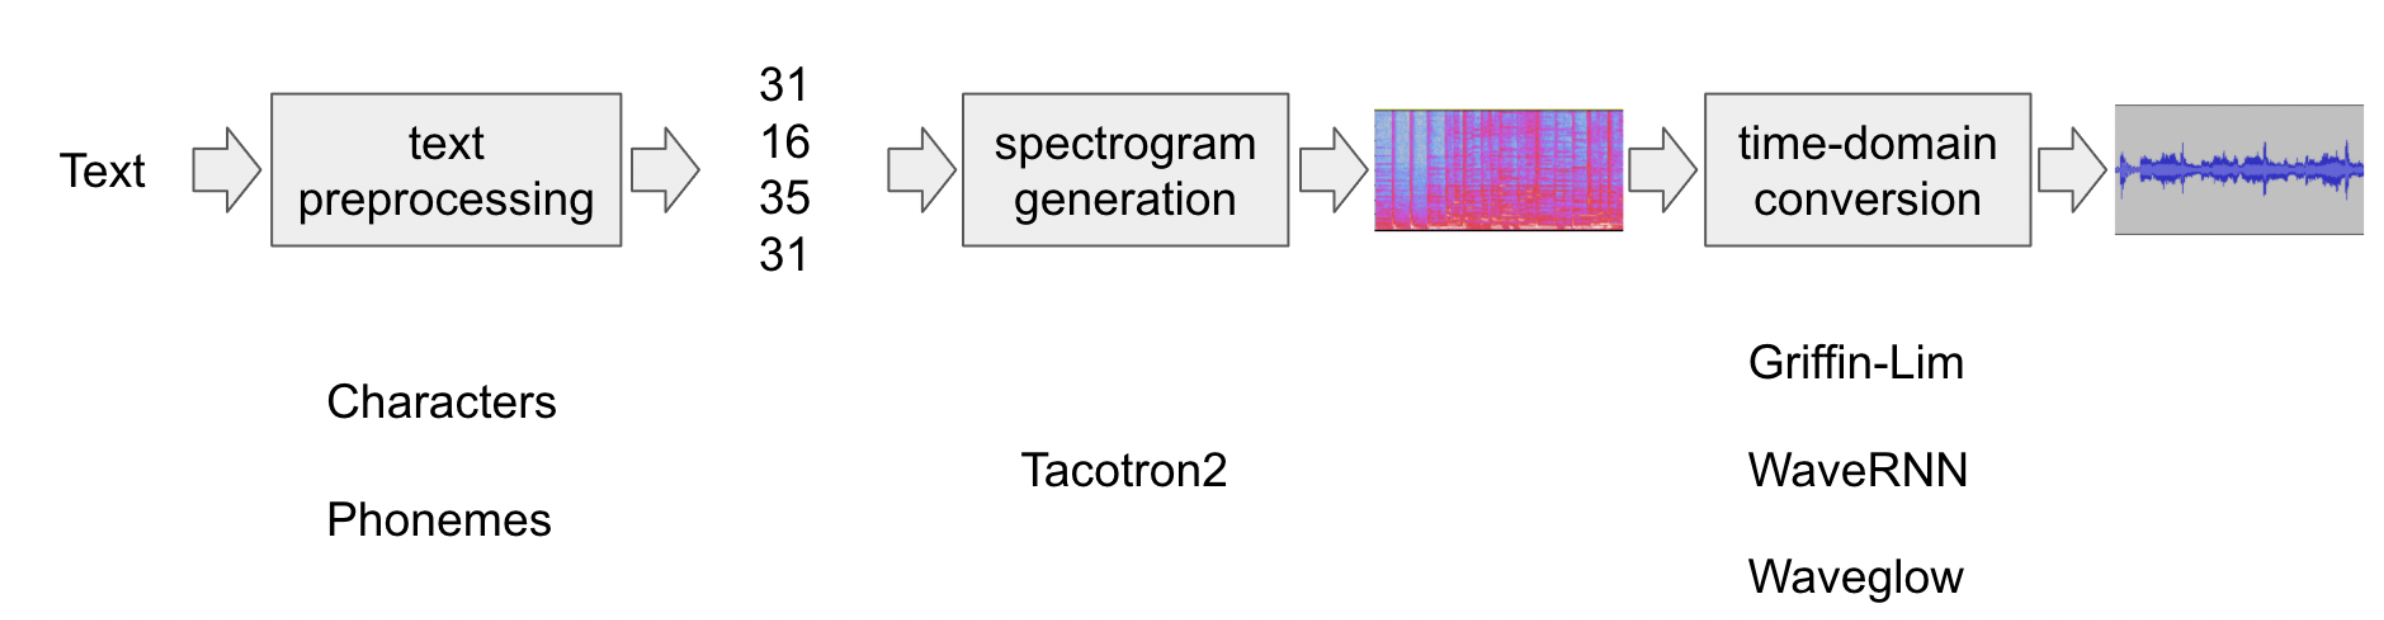
\includegraphics[width=0.99\linewidth]{figs/tts_pipeline.png}
    	\caption{Base pipeline of Text-to-speech task}
    \end{figure}
    
    Datasets: LJSpeech, LibriTTS, CommonVoice, OpenTTS (Ru)
    
    \myfootnotewithlink{https://pytorch.org/audio/stable/tutorials/tacotron2_pipeline_tutorial.html}{Text-to-speech with Tacotron2 pytorch tutorial}

\end{frame}
%=======
\begin{frame}{TTS: quality}
    \begin{itemize}
        \item Quality: Subjective perception
        \item Overall impression, Intelligibility, Similarity, Naturalness, Pleasantness, Intonation and pauses, Emotions, Listening effort

        \item Mean Opinion Score (MOS): Crowdsourcing by Yandex Toloka/Amazon
        $$\text{MOS}={\frac{\sum_{n=1}^{N}{\cal R}_{n}}{N}}$$
        \begin{figure}
        	\centering
        	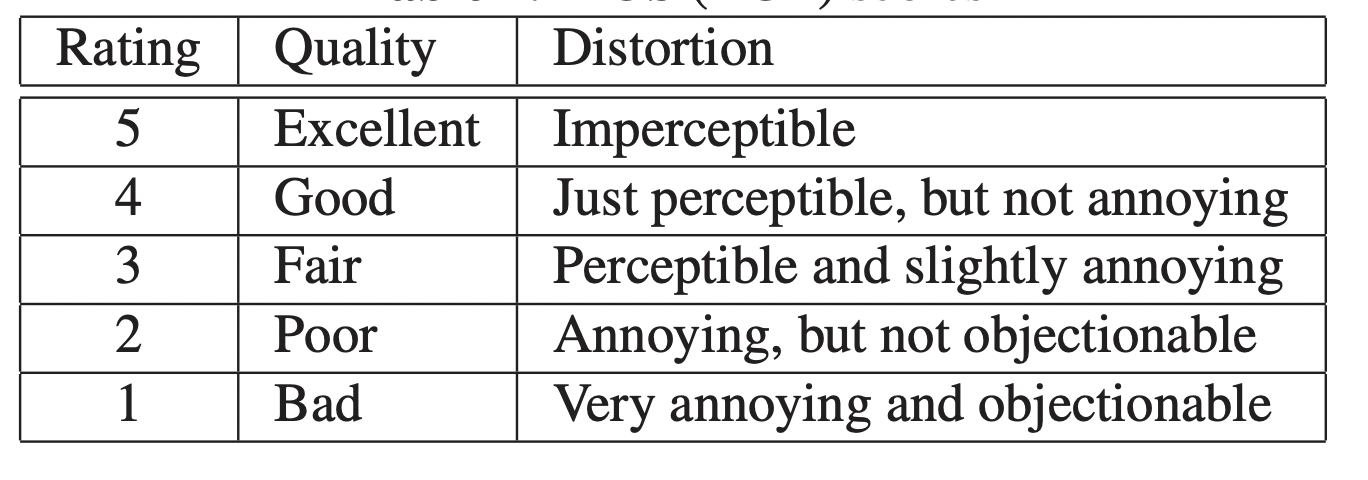
\includegraphics[width=0.75\linewidth]{figs/mos.png}
        \end{figure}
        \item Side-by-Side audio comparison (evaluate small improvements)
    \end{itemize}
\end{frame}

%=======
\section{Attention ideas in TTS}
%=======
\begin{frame}{Tacotron 2}
    \begin{figure}
    	\centering
    	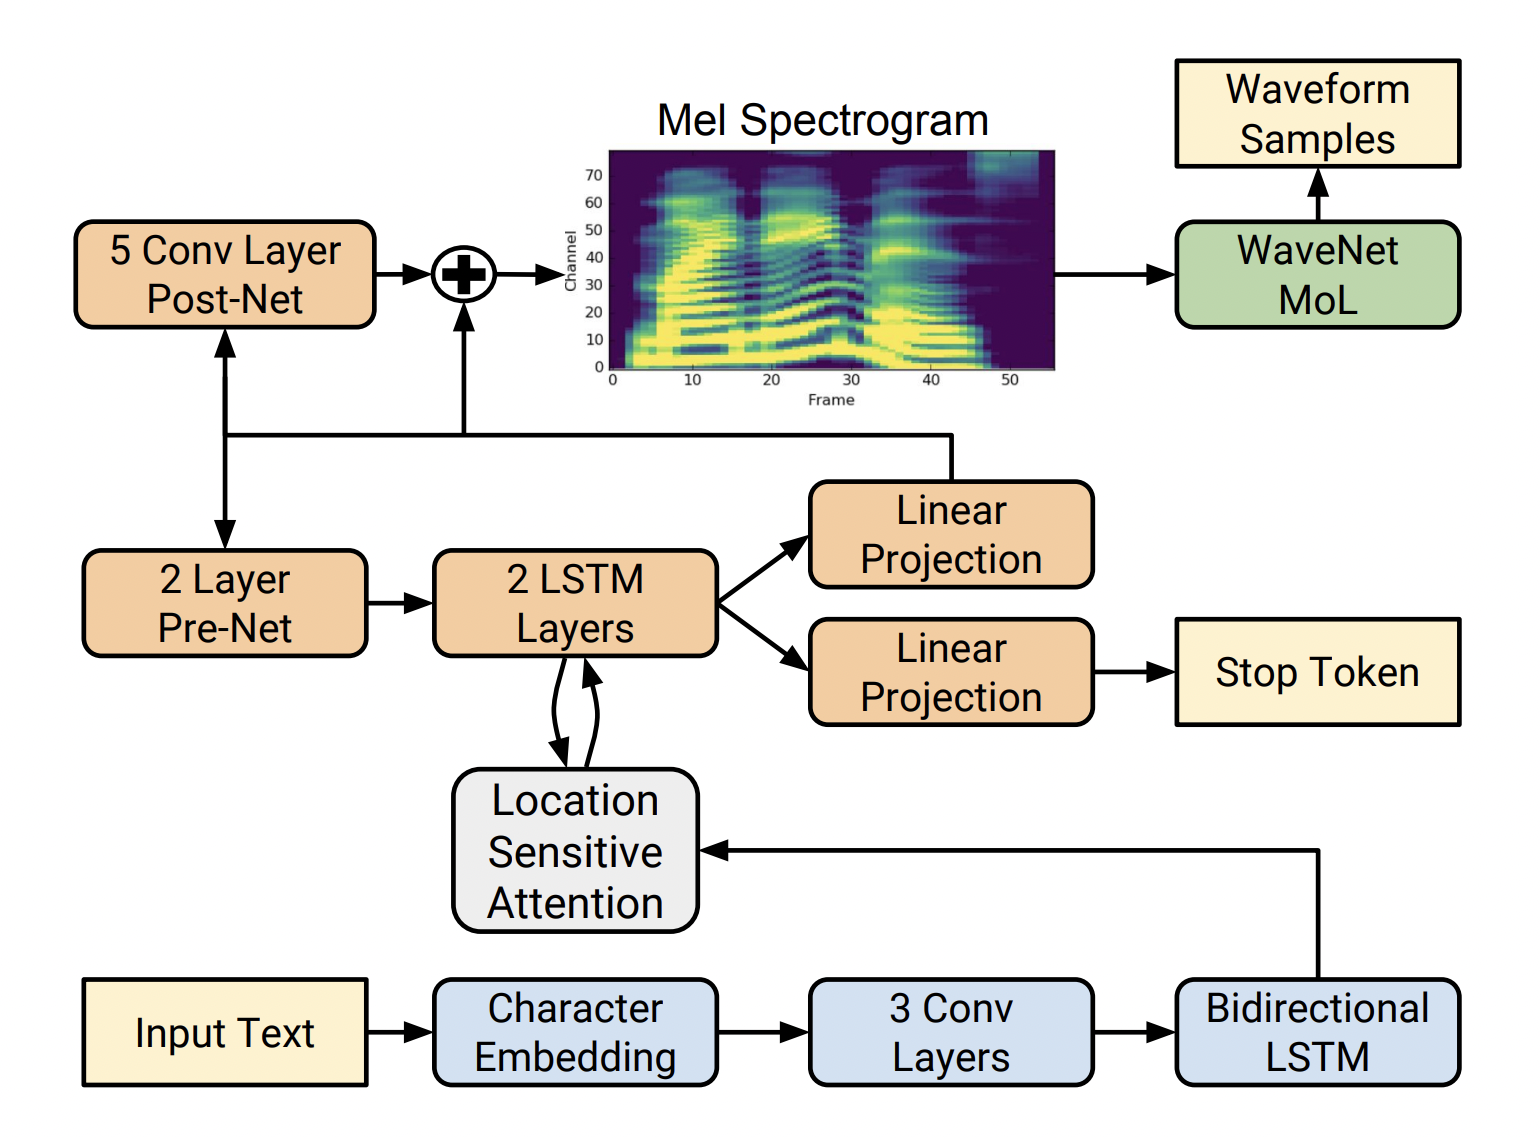
\includegraphics[width=0.75\linewidth]{figs/tacotron2.png}
    	\caption{Recurrent seq-to-seq feature prediction network with attention that maps character embeddings to spectrograms, followed by a modified WaveNet to synthesize time-domain waveforms}
    \end{figure}
    
    \myfootnotewithlink{https://arxiv.org/pdf/1712.05884.pdf}{Shen et al., Natural TTS Synthesis by Conditioning Wavenet on MEL Spectrogram Predictions, 2018 IEEE ICASSP}

\end{frame}
%=======
\begin{frame}{Tacotron 2: text Encoder}
    \begin{figure}
    	\centering
    	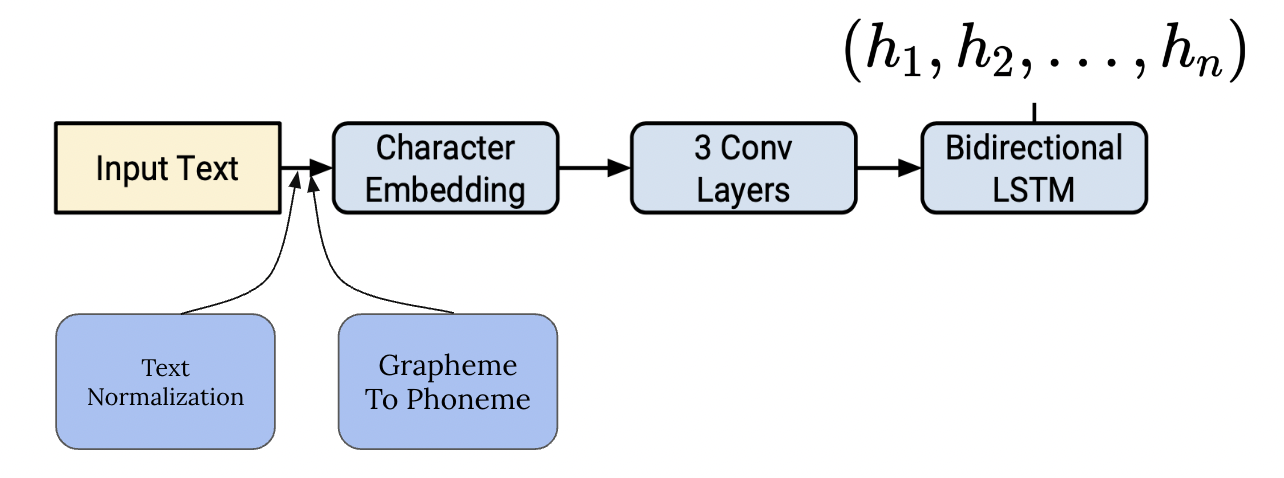
\includegraphics[width=0.99\linewidth]{figs/tacotron_text_encoder.png}
    \end{figure}
    
    \myfootnotewithlink{https://github.com/markovka17/dla/tree/2020}{HSE DLA course}

    
\end{frame}
%=======
\begin{frame}{Tacotron 2}
    \begin{figure}
    	\centering
    	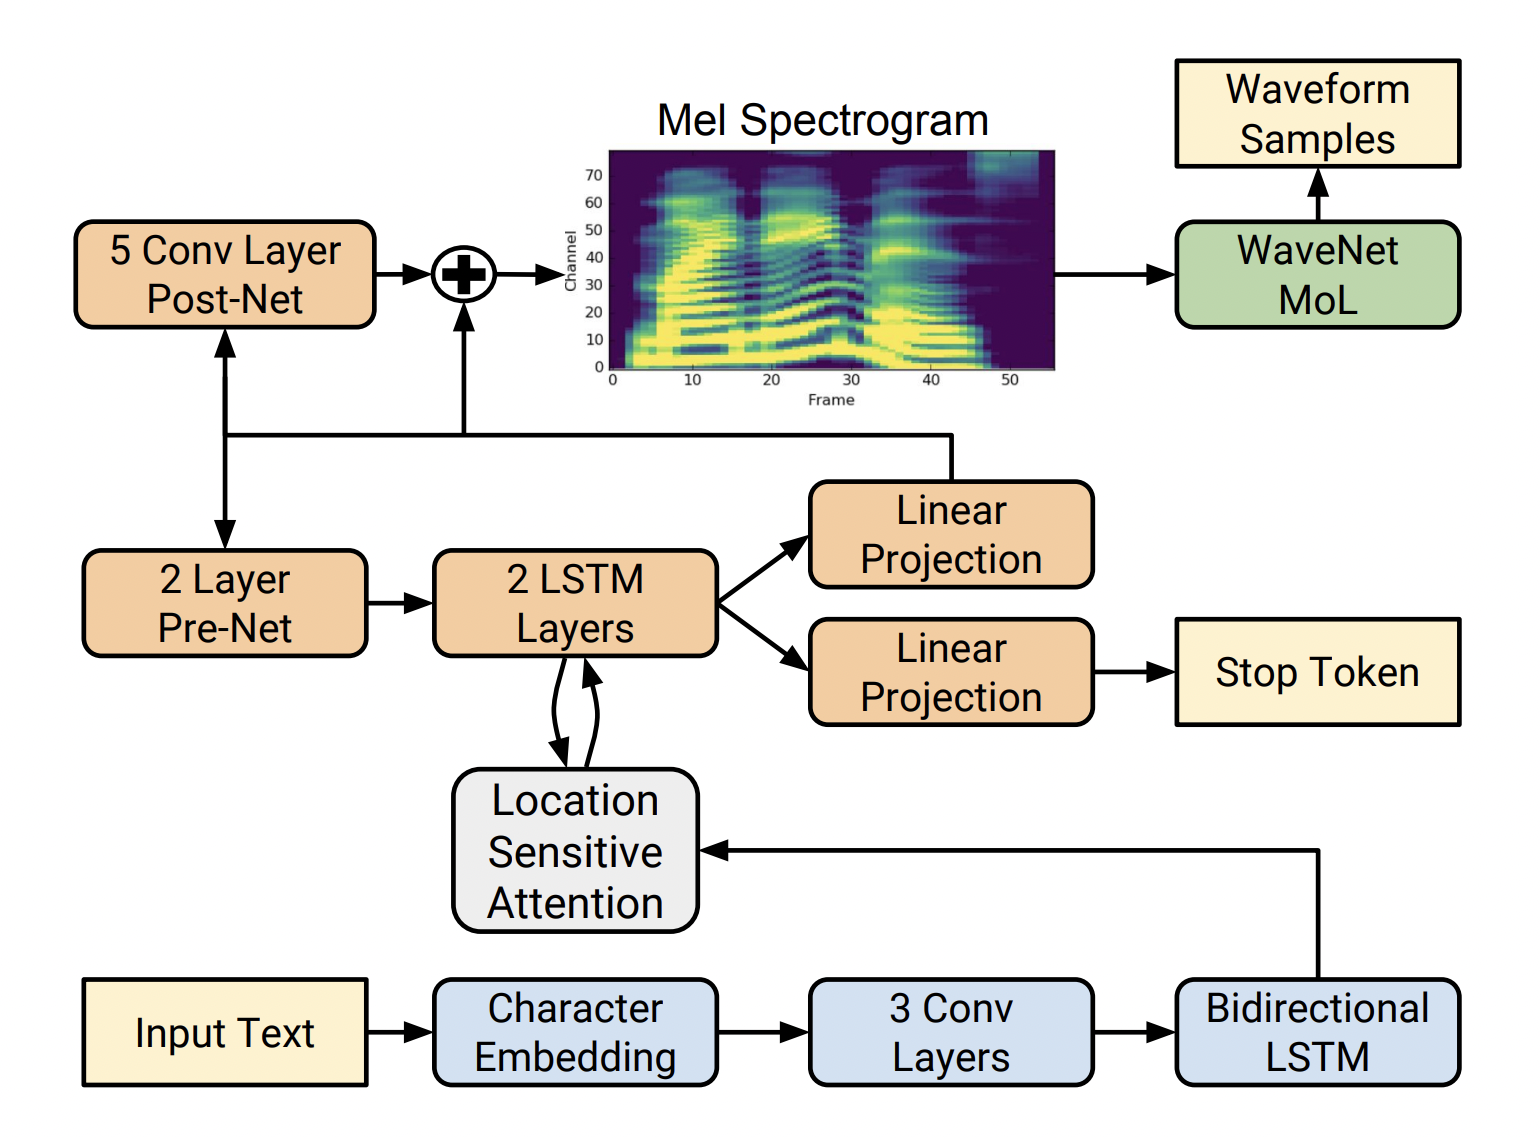
\includegraphics[width=0.6\linewidth]{figs/tacotron2.png}
    \end{figure}
    
    $$\mathcal{L}=\mathcal{L}_{\mathrm{pre}}+\mathcal{L}_{\mathrm{post}}+\mathrm{StopToken}$$
    $$\mathcal{L}_{\mathrm{pre}}=\mathrm{MSE}(x,\hat{x}_{\mathrm{pre}})$$
    $$\mathcal{L}_{\mathrm{post}}=\mathrm{MSE}(x,\hat{x}_{\mathrm{post}})$$
    $$\mathrm{StopToken}=\mathrm{CE}(a,\mathcal{I}[h=\mathrm{Stop}])$$


\end{frame}
%=======
\begin{frame}{Guided Attention}
\begin{itemize}
    \item Idea: text position $n$ progresses nearly linearly to the time $t$: $$n \sim at, ~ a \sim N/T$$
    \item Add loss $\mathcal{L}_{\mathrm{att}}\left(A\right)=\mathbb{E}_{n t}[A_{n t}W_{n t}],$ where $W_{n t}=1-\exp\{-(n/N-t/T)^{2}/2g^{2}\}, ~~g = 0.2, ~~A \in \mathbb{R}^{N \times T}$
\end{itemize}
    \begin{figure}
    	\centering
    	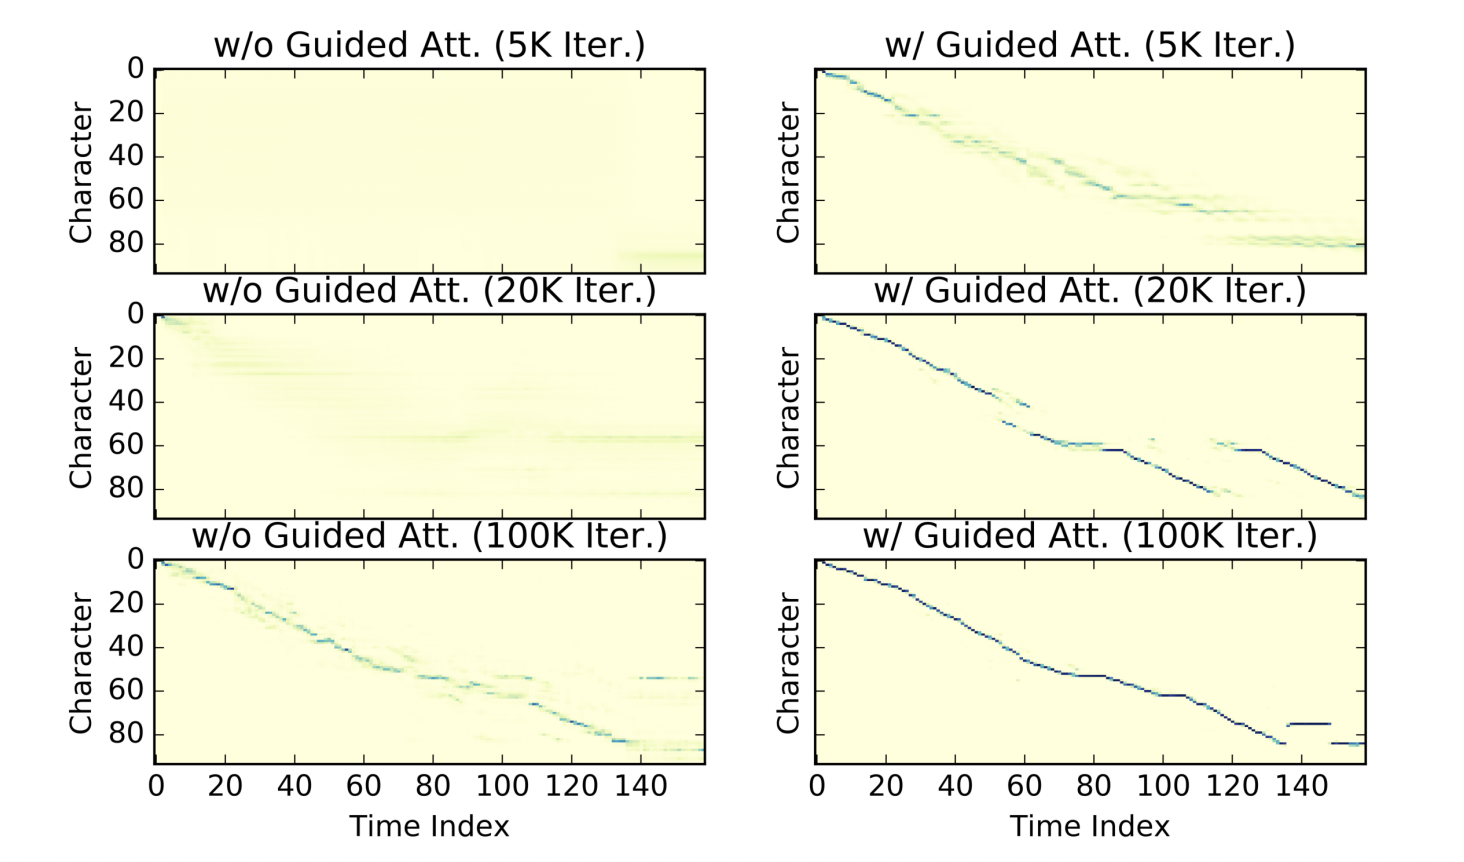
\includegraphics[width=0.6\linewidth]{figs/guided_attention.png}
    	\caption{Comparison of the attention matrix A, trained with (Right) and without (Left) the guided attention loss }
    \end{figure}
    
    \myfootnotewithlink{https://arxiv.org/pdf/1710.08969.pdf}{Tachibanaet al., Efficiently Trainable Text-to-Speech System Based on Deep Convolutional Networks with Guided Attention, 2018 IEEE ICASSP}

\end{frame}
%=======
\begin{frame}{Monotonic Attention}
For $j=t_{i-1},t_{i-1}+1,t_{i-1}+2,\dots$:
\begin{array}{l c r}{{e_{i,j}=a(s_{i-1},h_{j})}}\\ {{p_{i,j}=\sigma(e_{i,j})}}\\ {{z_{i,j}\sim\mathrm{Bernoulli}(p_{i,j})}}
\end{array}
\\where $a(\cdot)$ -- learnable deterministic "energy function", $\sigma(\cdot)$ -- logistic sigmoid function
    \begin{figure}
    	\centering
    	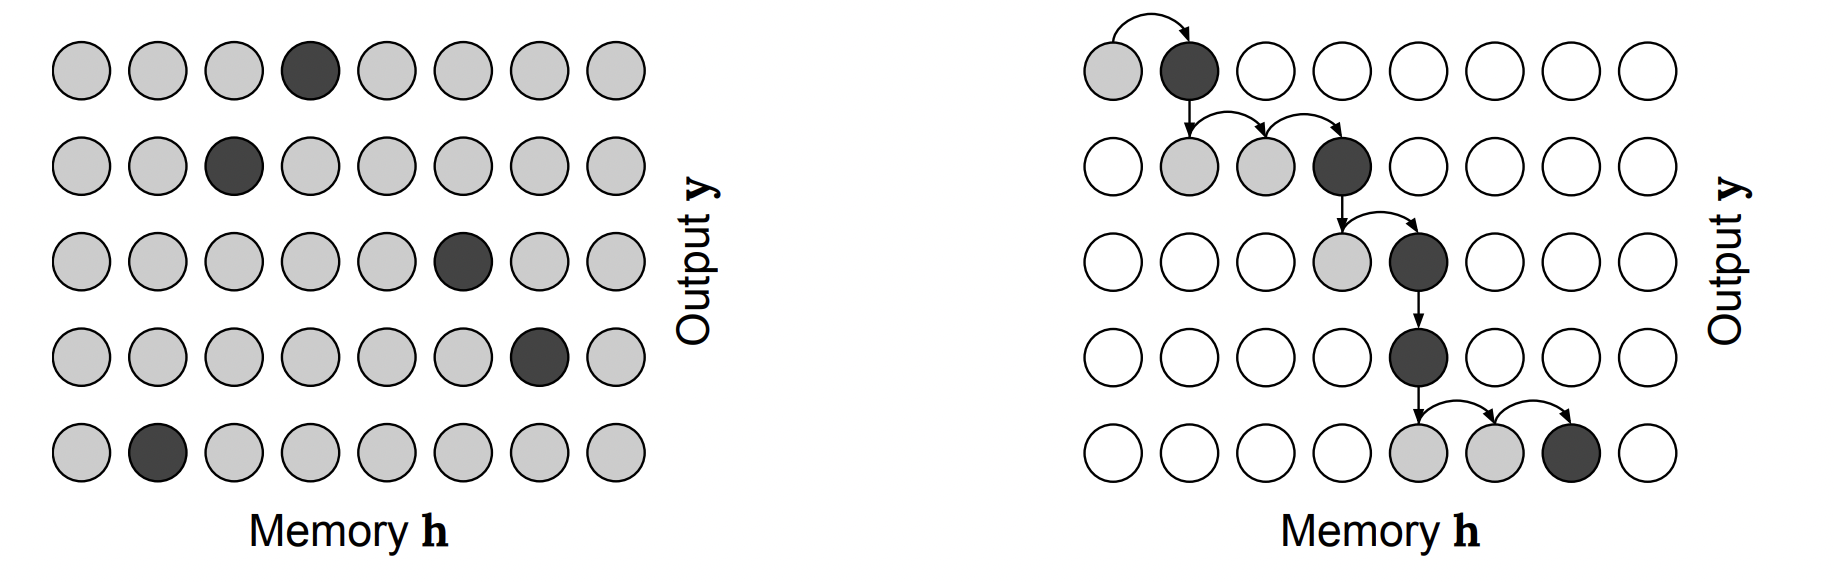
\includegraphics[width=0.8\linewidth]{figs/monotonic_attention.png}
    	\caption{Left: schematic of the stochastic process underlying softmax-based attention decoders. Right: monotonic stochastic decoding process.}
    \end{figure}
    
    \myfootnotewithlink{https://arxiv.org/pdf/1704.00784.pdf}{Raffel et al., Online and Linear-Time Attention by Enforcing Monotonic Alignments, Algorithms, A.G., 2017}

\end{frame}
%=======
\begin{frame}{Global Style Token (GST)}
    \begin{figure}
    	\centering
    	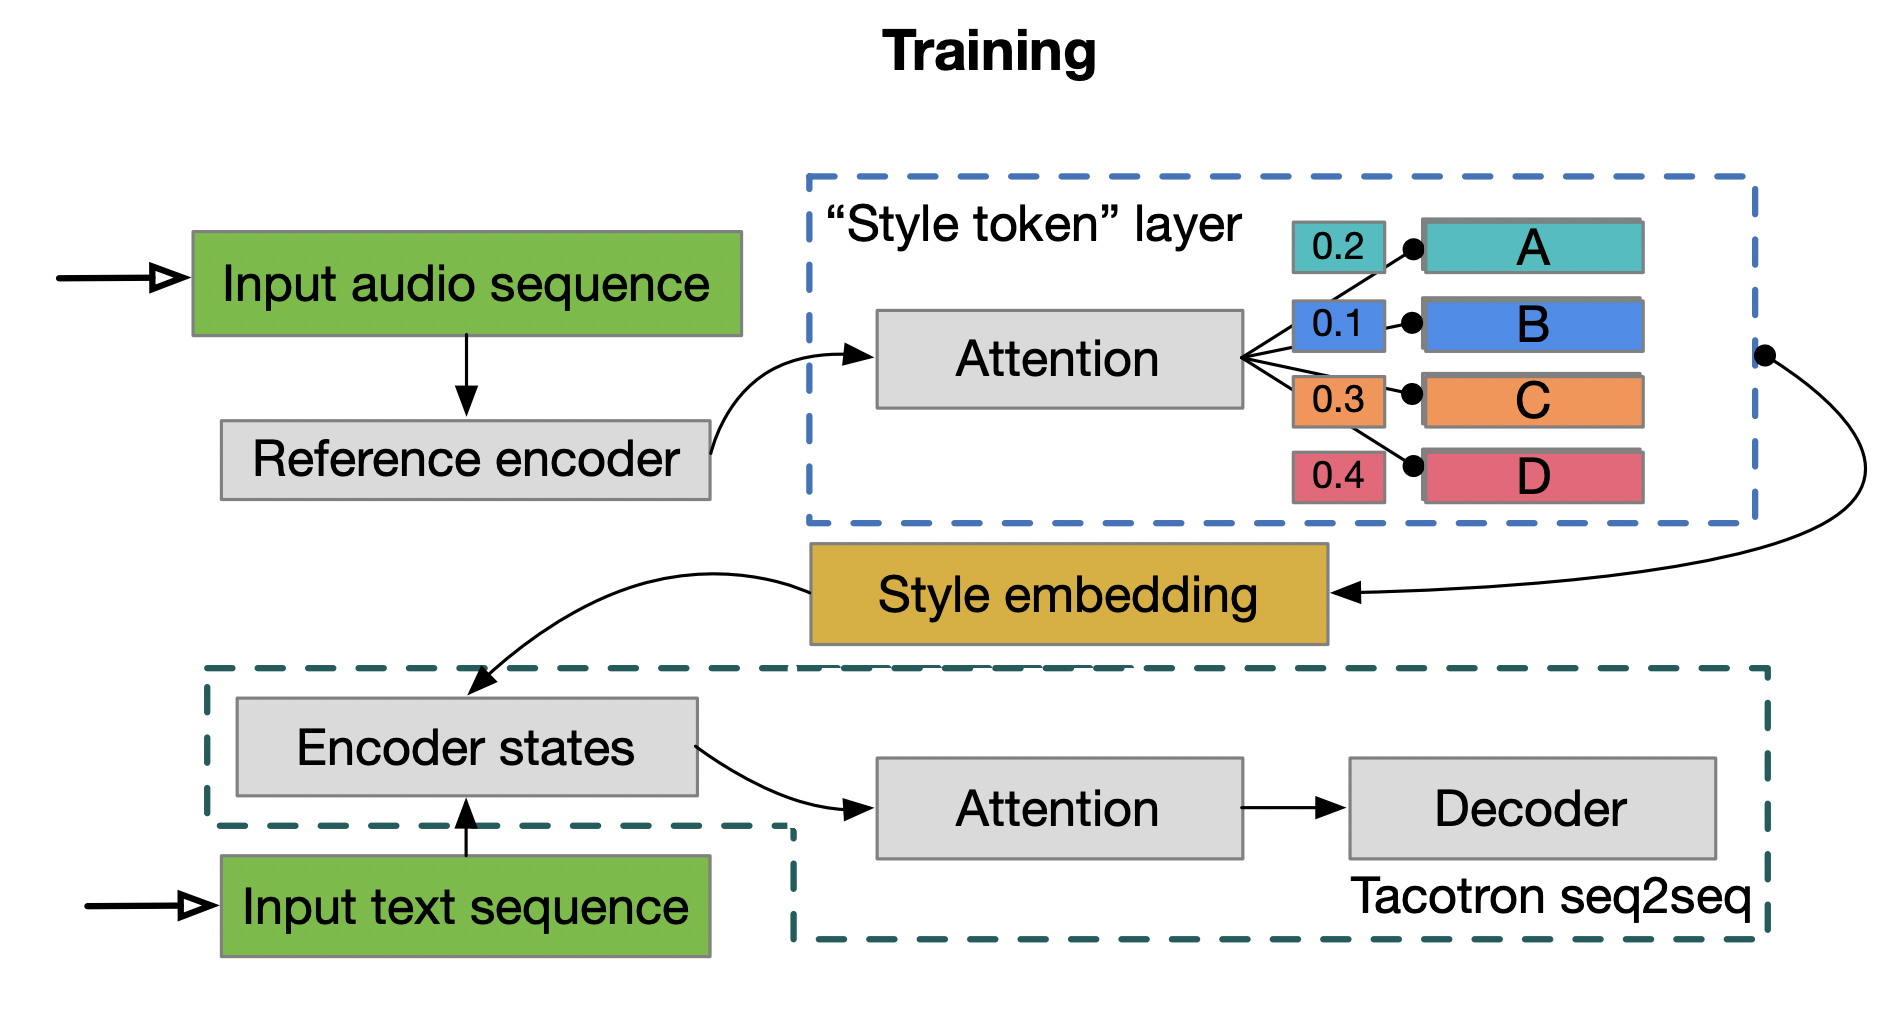
\includegraphics[width=0.99\linewidth]{figs/gst_train.png}
    	\caption{Log-mel spectrogram of the training target is fed to the reference encoder followed by a style token layer. The resulting style embedding is used to condition the Tacotron text encoder states}
    \end{figure}
    
    \myfootnotewithlink{https://arxiv.org/pdf/1803.09017.pdf}{Wang et al., Style Tokens: Unsupervised Style Modeling, Control and Transfer in End-to-End Speech Synthesis, International Conference on Machine Learning, 2018}

\end{frame}
%=======
\begin{frame}{Global Style Token (GST)}
    \begin{figure}
    	\centering
    	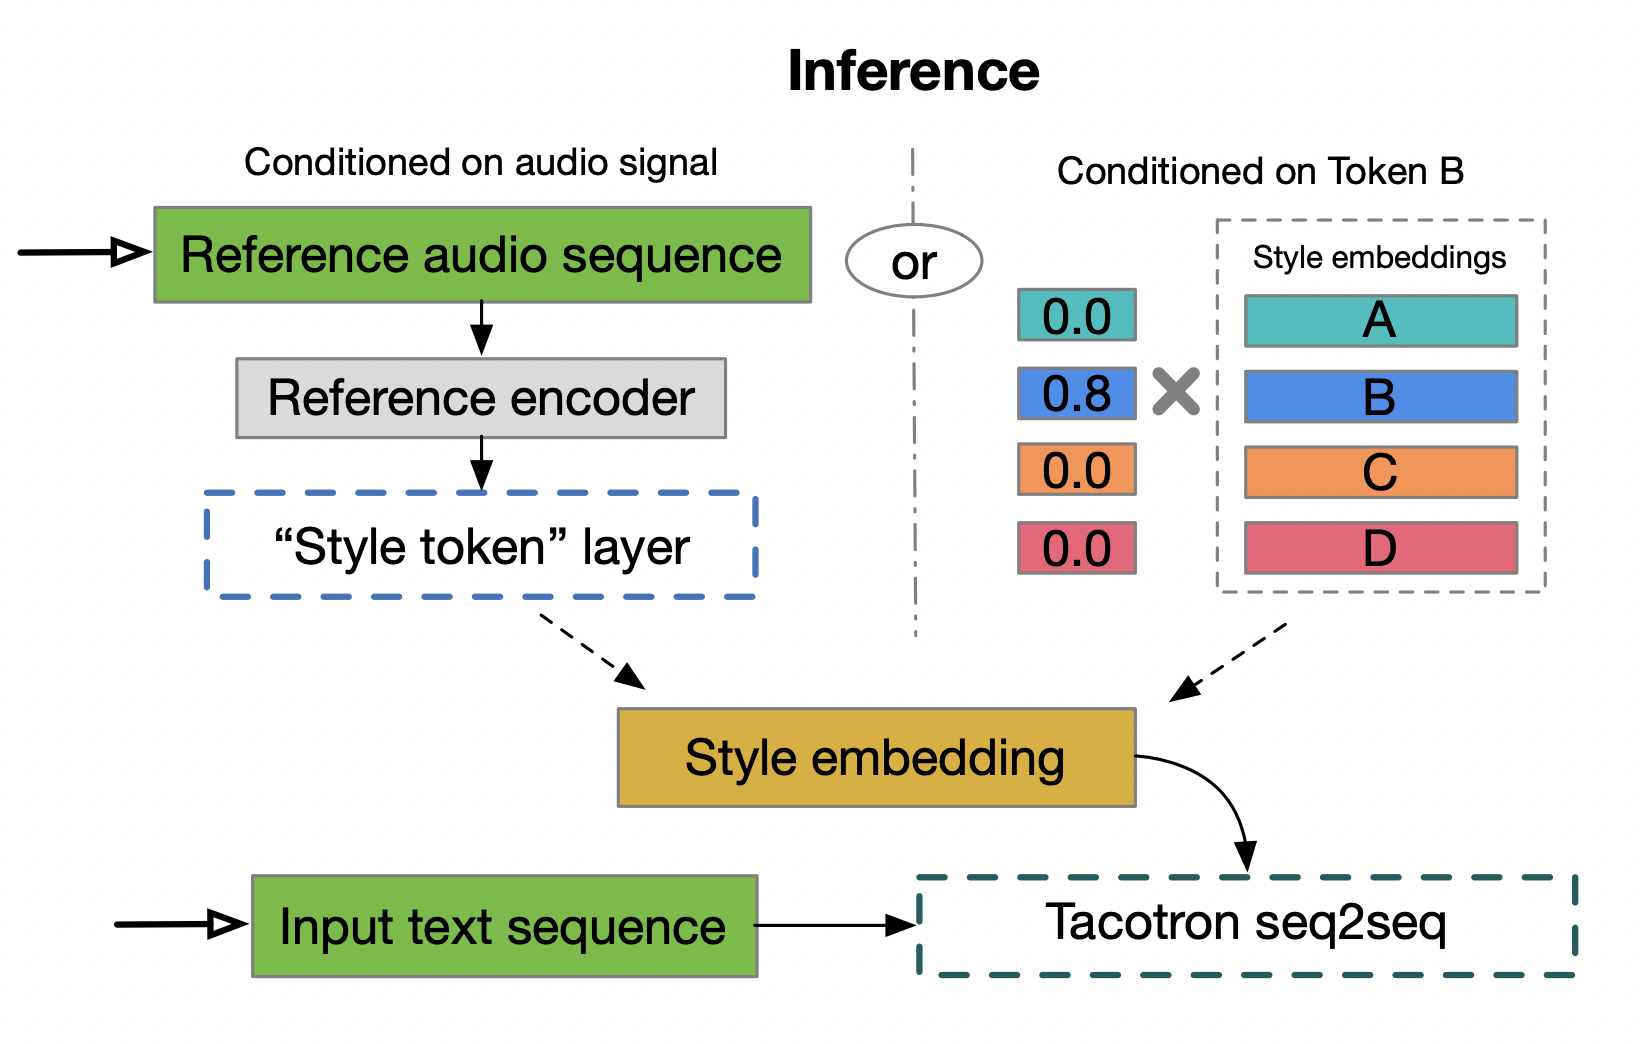
\includegraphics[width=0.8\linewidth]{figs/gst_infer.png}
    	\caption{Inference: can feed an arbitrary reference signal to synthesize text with its speaking style. Alternatively, can remove the reference encoder and directly control synthesis using the learned interpretable tokens.}
    \end{figure}
    
    \myfootnotewithlink{https://arxiv.org/pdf/1803.09017.pdf}{Wang et al., Style Tokens: Unsupervised Style Modeling, Control and Transfer in End-to-End Speech Synthesis, International Conference on Machine Learning, 2018}

\end{frame}

%=======
\section{SOTA TTS models}
%=======
\begin{frame}{DeepVoice}
    \begin{figure}
    	\centering
    	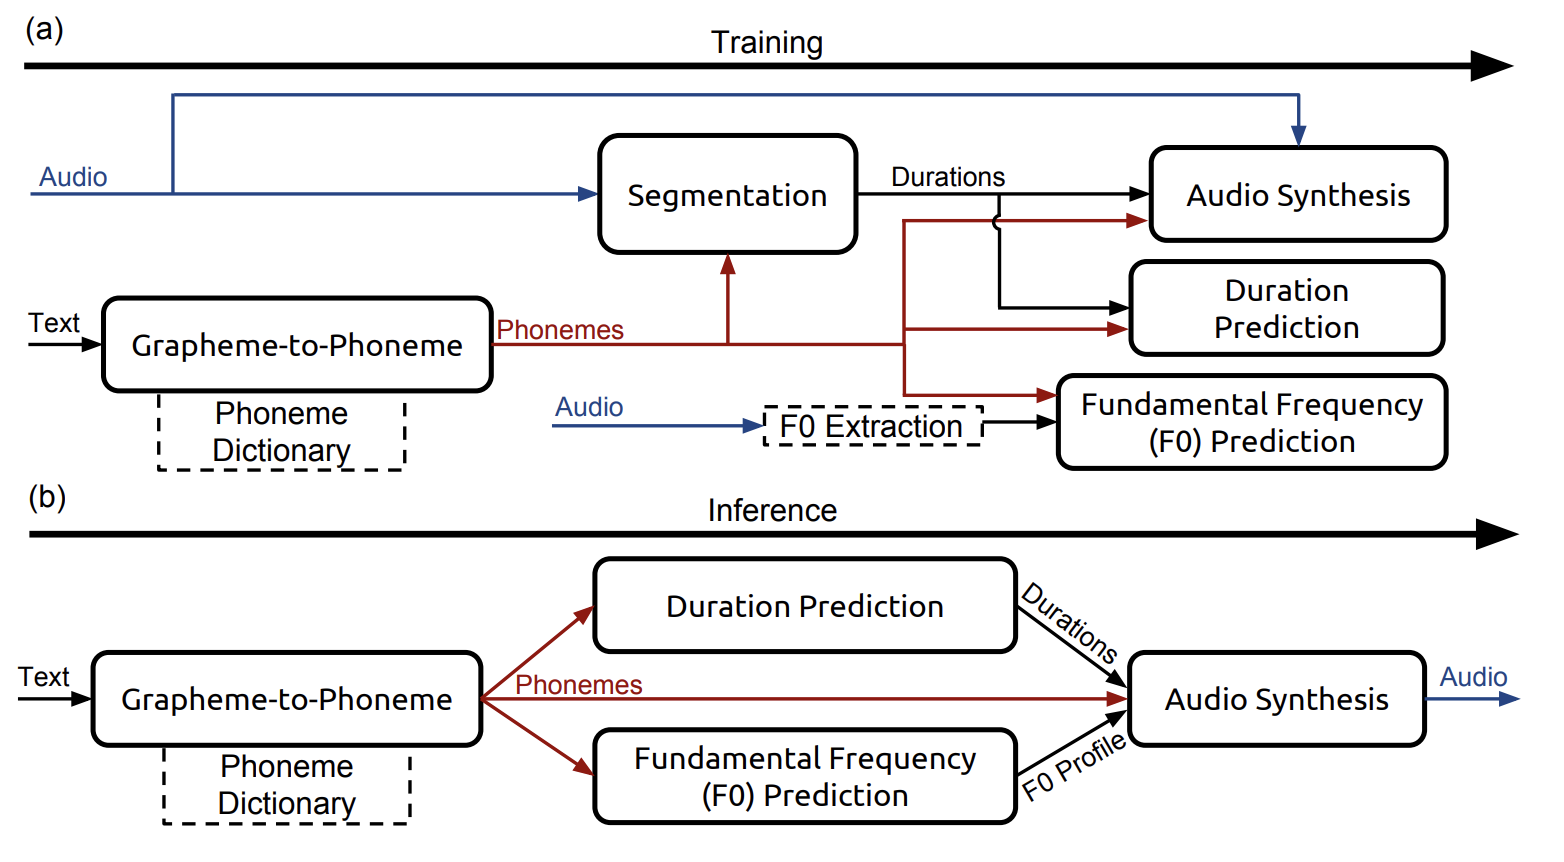
\includegraphics[width=0.9\linewidth]{figs/deepvoice.png}
    \end{figure}
    \begin{itemize}
        \item Grapheme-to-phoneme model -- for words not present in a phoneme dictionary
        \item Segmentation model identifies where in the audio each phoneme begins and ends
    \end{itemize}
    \myfootnotewithlink{https://arxiv.org/pdf/1702.07825.pdf}{Arik et al., Deep Voice: Real-time Neural Text-to-Speech, ArXiv preprint, 2017}
\end{frame}
%=======
\begin{frame}{FastSpeech}
    \begin{figure}
    	\centering
    	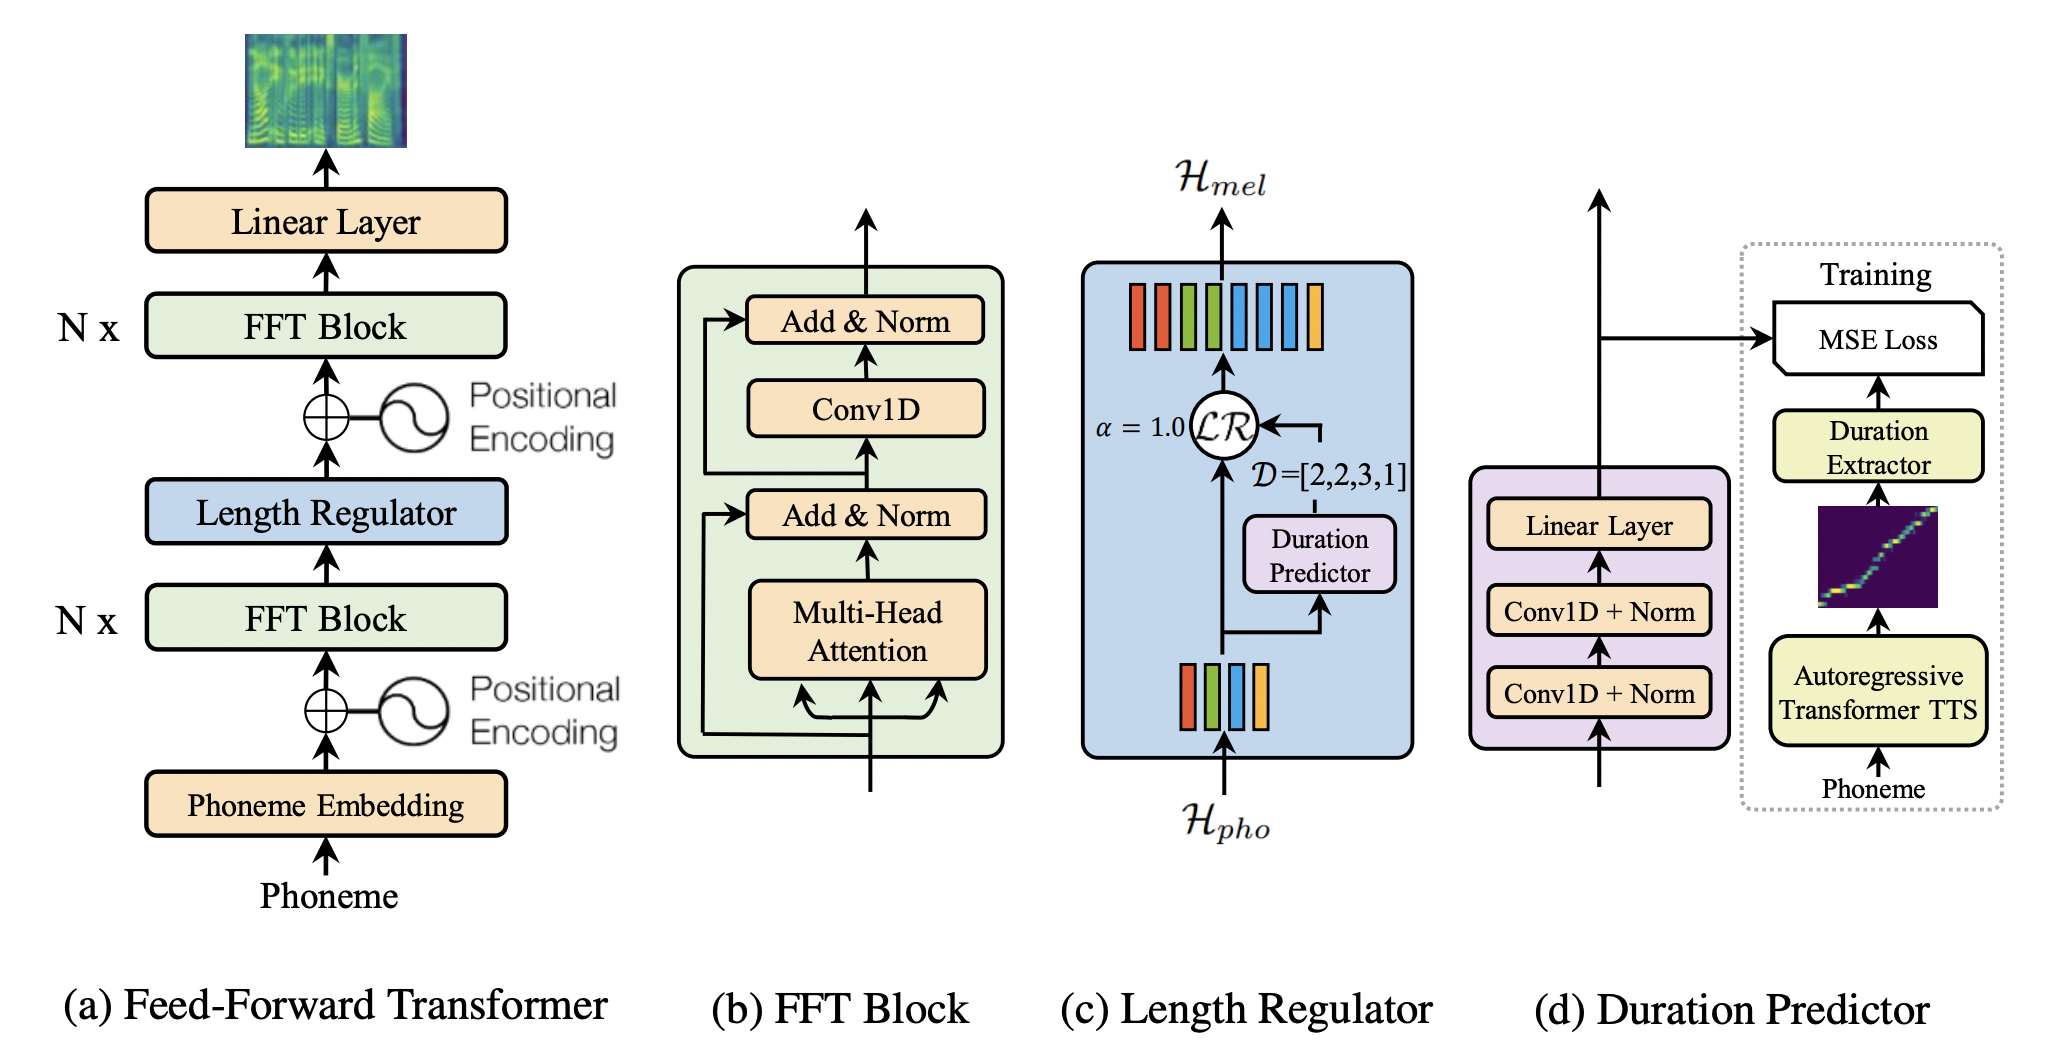
\includegraphics[width=0.93\linewidth]{figs/fastspeech.png}
    \end{figure}
    \begin{itemize}
        \item Use of feed-forward Transformer (FFT) blocks
        \item Extract attention alignments from an encoder-decoder based teacher model for phoneme duration prediction
    \end{itemize}
    \myfootnotewithlink{https://arxiv.org/pdf/1905.09263.pdf}{Yi et al., FastSpeech: fast, robust and controllable text to speech, Proceedings of the 33rd International Conference on NIPS, 2019}

\end{frame}
%=======
\begin{frame}{FastSpeech vs Tacotron}
\begin{table}[]
\begin{tabular}{|c|c|c|}
\hline
                                                                                                        & \textbf{Tacotron}                                                                    & \textbf{Fastspeech}                                                    \\ \hline
\textbf{Inference speed}                                                                                & Slow                                                                                 & Fast                                                                   \\ \hline
\textbf{\begin{tabular}[c]{@{}c@{}}Synthesized \\ speech is robust?\end{tabular}}                       & \begin{tabular}[c]{@{}c@{}}No, some words \\ are skipped or \\ repeated\end{tabular} & Yes                                                                    \\ \hline
\textbf{\begin{tabular}[c]{@{}c@{}}Controllability \\ (voice speed or \\ prosody control)\end{tabular}} & Lack                                                                                 & \begin{tabular}[c]{@{}c@{}}Adjust voice \\ speed smoothly\end{tabular} \\ \hline
\end{tabular}
\end{table}

\end{frame}
%=======
\begin{frame}{FastSpeech 2}
    \begin{figure}
    	\centering
    	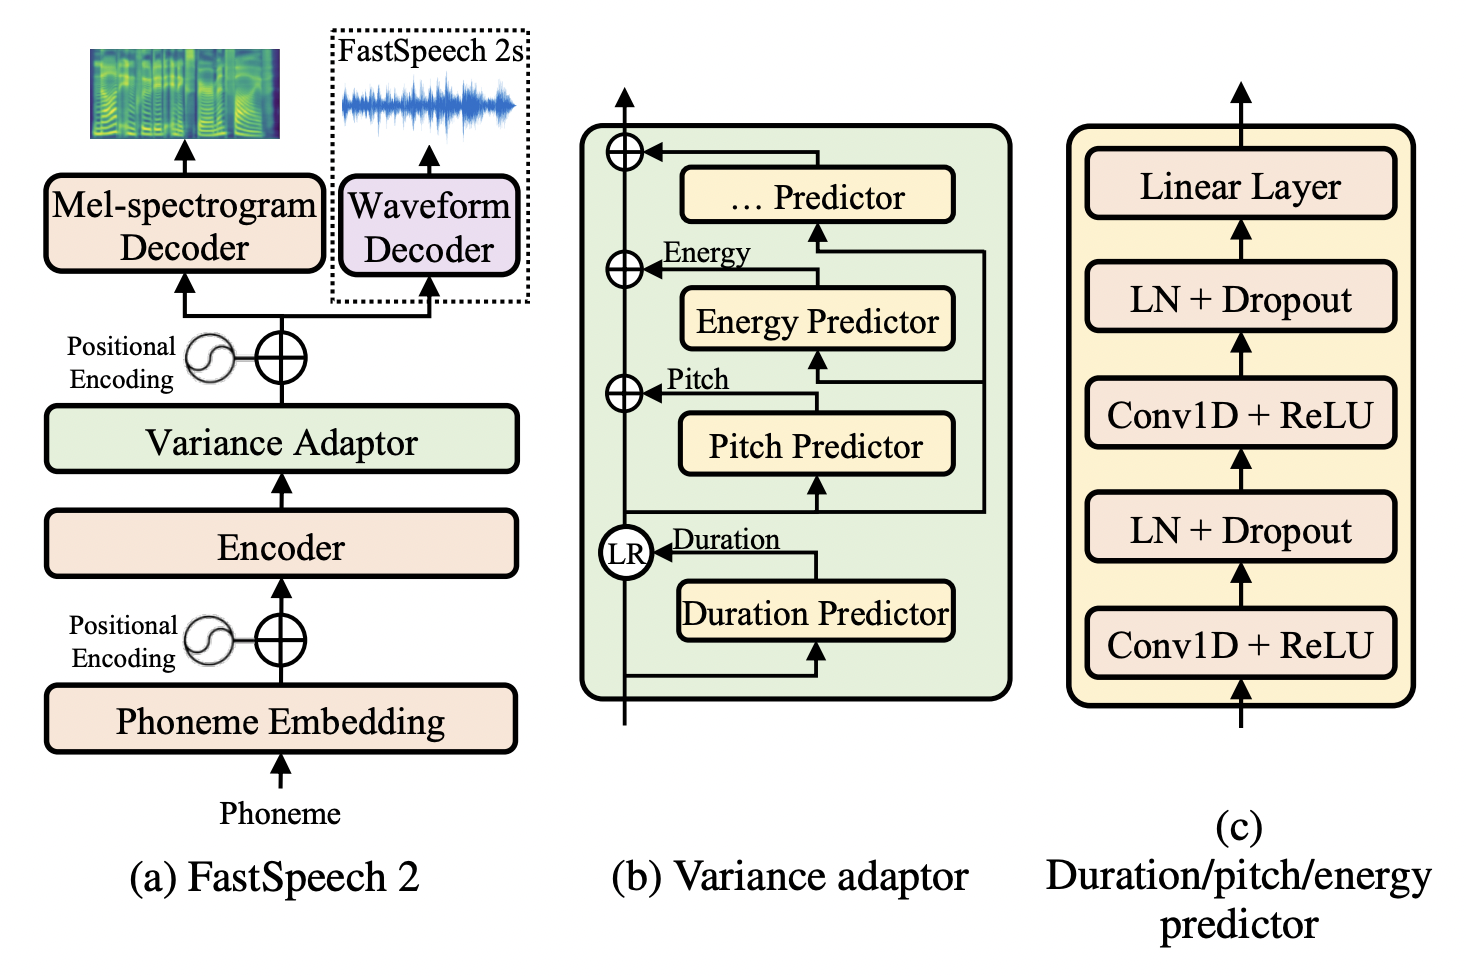
\includegraphics[width=0.72\linewidth]{figs/fastspeech2.png}
    \end{figure}
    \begin{itemize}
        \item Directly training the model with ground-truth target instead of the simplified output from teacher
        \item more information of speech used as conditional inputs: duration, pitch (emotions), energy (volume and prosody)
    \end{itemize}

    \myfootnotewithlink{https://arxiv.org/pdf/2006.04558.pdf}{Ren, Yi et al. FastSpeech 2: Fast and High-Quality End-to-End Text to Speech, Arxiv preprint, 2021}

\end{frame}
%=======
\begin{frame}{AdaSpeech}
    \begin{figure}
    	\centering
    	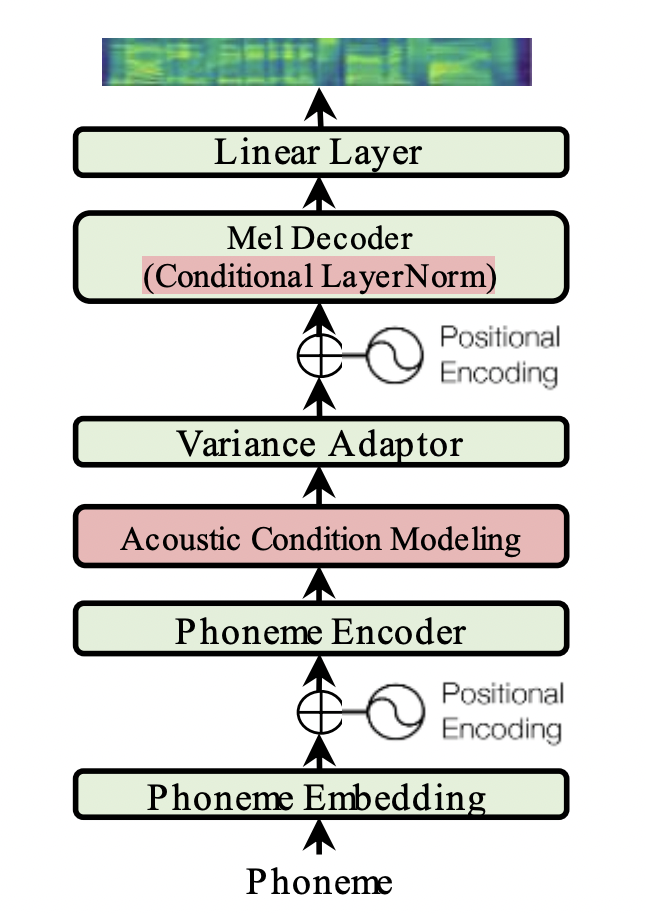
\includegraphics[width=0.4\linewidth]{figs/adaspeech.png}
    \end{figure}
    \begin{itemize}
        \item Adopted FastSpeech 2
        \item Add acoustic condition modeling
    \end{itemize}
    \myfootnotewithlink{https://arxiv.org/pdf/2103.00993.pdf}{Chen et al., AdaSpeech: Adaptive Text to Speech for Custom Voice, Arxiv preprint, 2021}

\end{frame}
%=======
\begin{frame}{AdaSpeech: acoustic condition modeling}
    \begin{figure}
    	\centering
    	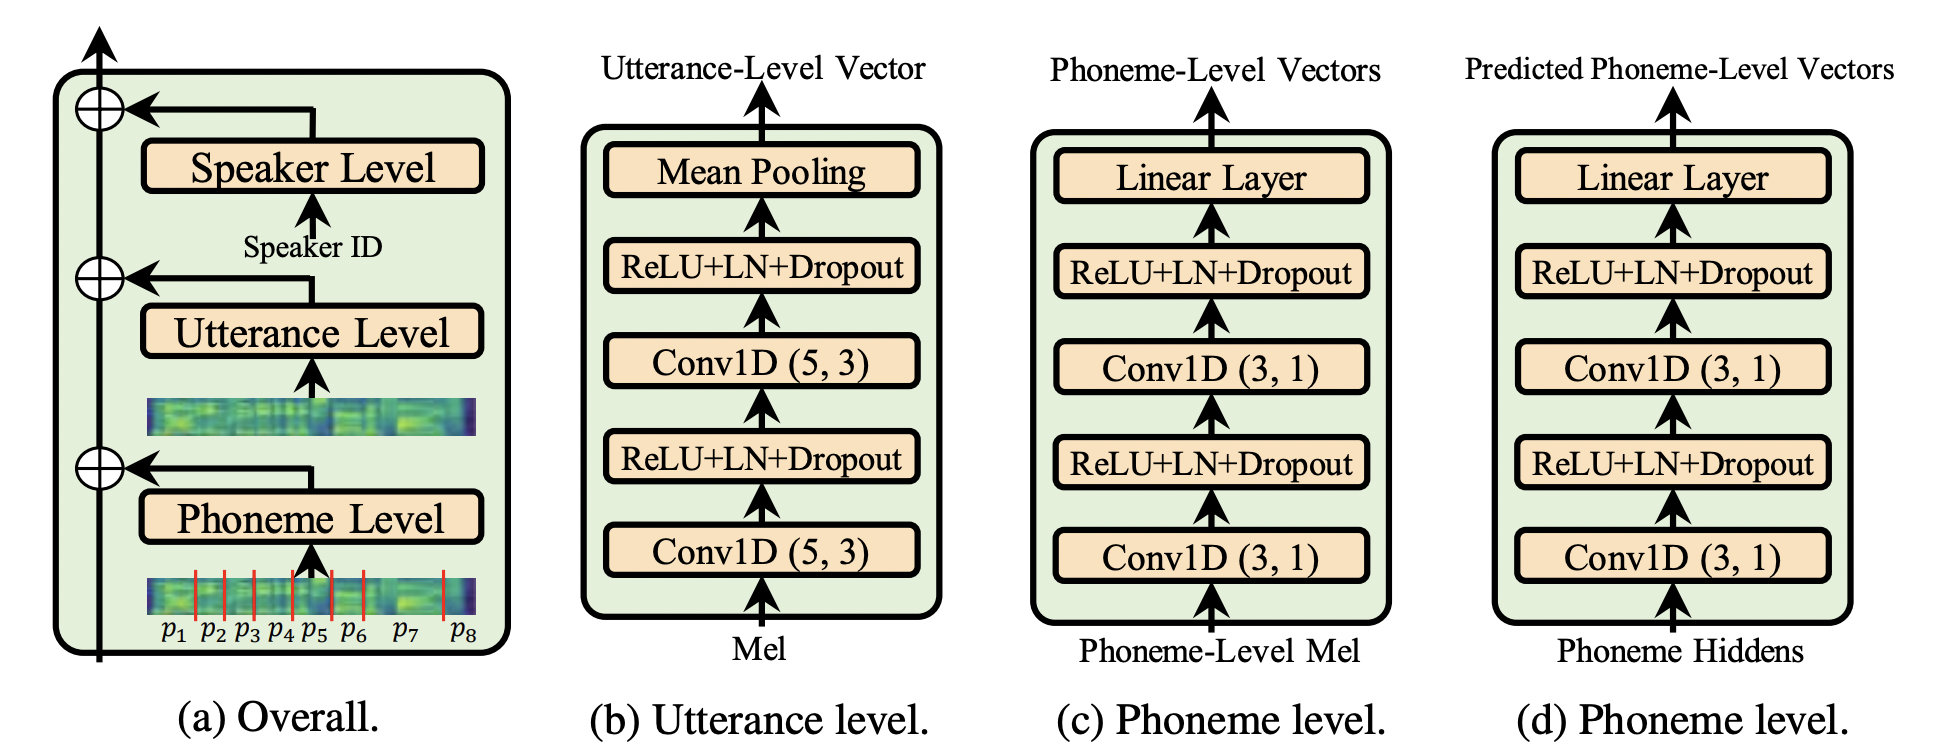
\includegraphics[width=0.99\linewidth]{figs/adaspeech_acoustic.png}
    	\caption{Adding acoustic conditions such as speaker timbre, prosody and recording environments into model}
    \end{figure}
    
    \myfootnotewithlink{https://arxiv.org/pdf/2103.00993.pdf}{Chen et al., AdaSpeech: Adaptive Text to Speech for Custom Voice, Arxiv preprint, 2021}

\end{frame}

\end{document} 
